
%%%%%%%%%%%%%%%%%%%%%%%%%%%%%%%%%%%%%%%%
%          Transmission
%%%%%%%%%%%%%%%%%%%%%%%%%%%%%%%%%%%%%%%%

\section{Transmission Design}
\label{sec:transmissionDesign}

The actuator design philosophy is to make high power actuators with the capability of interacting with the environment. Namely, the actuator should not be stiff as the heavily geared motors, which are widely used in industrial robots. Instead, it should be back-drivable meaning that the torque applied at the output shaft should be felt at the input shaft. The benefits are threefold, firstly, back-drivability prevents geatboxes from being damaged by external forces; second, it allows for proprioceptive sensing\cite{Seok2012}; thirdly, allows for fast dynamics in legged locomotion.

After the motor selection and gear ratio is determined from previous sections, focus was put on how to design the transmission system so that it can achieve the desired gear ratio while satisfying dimensional constraints.

\subsection{Transmission Design Comparison}
\label{sec:transmissionComparison}

\textbf{Harmonic drive} is composed of the wave generator, flexspline and circular spline. It could provide high gear ratio typically between 30:1 to 200:1 with zero backlash. Harmonic drive is employed by the quadrupedal robot starlETH\cite{Hutter2013} and the bipedal robot ATRIAS\cite{Hubicki2016}. However, harmonic drive is not back-drivable, which contradicts with our design paradigm.

\textbf{Cycloidal gearbox} has very low backlash and high torsional stiffness. It can operate quietly and withstand shock load. Bipedal robot Cassie uses cycloidal gearbox as the transmission. The drawback of cycloidal gearbox is that it requires customizing high precision parts.

\textbf{Single stage planetary gearbox} has high efficiency and the load could be distributed between planet gears, and standard gears are widely available at low cost. Nevertheless, no gear combination could provide the desired gear ratio for the given dimensional limitation with pitch of 0.4.

\textbf{Compound planetary gearboxes} have the benefits of single stage planetary gearboxes while providing more compact design for there are two stages for the planet gear. There are a range of gear teeth selection for the given dimensional limits. It is adopted as the transmission system design considering the dimensional limit and gear ratio requirement of the motor design.

\subsection{Compound Planetary Gearbox Design}
\label{sec:compoundGearBox}

\begin{figure}
	\centering
	\resizebox{1.0\linewidth}{!}{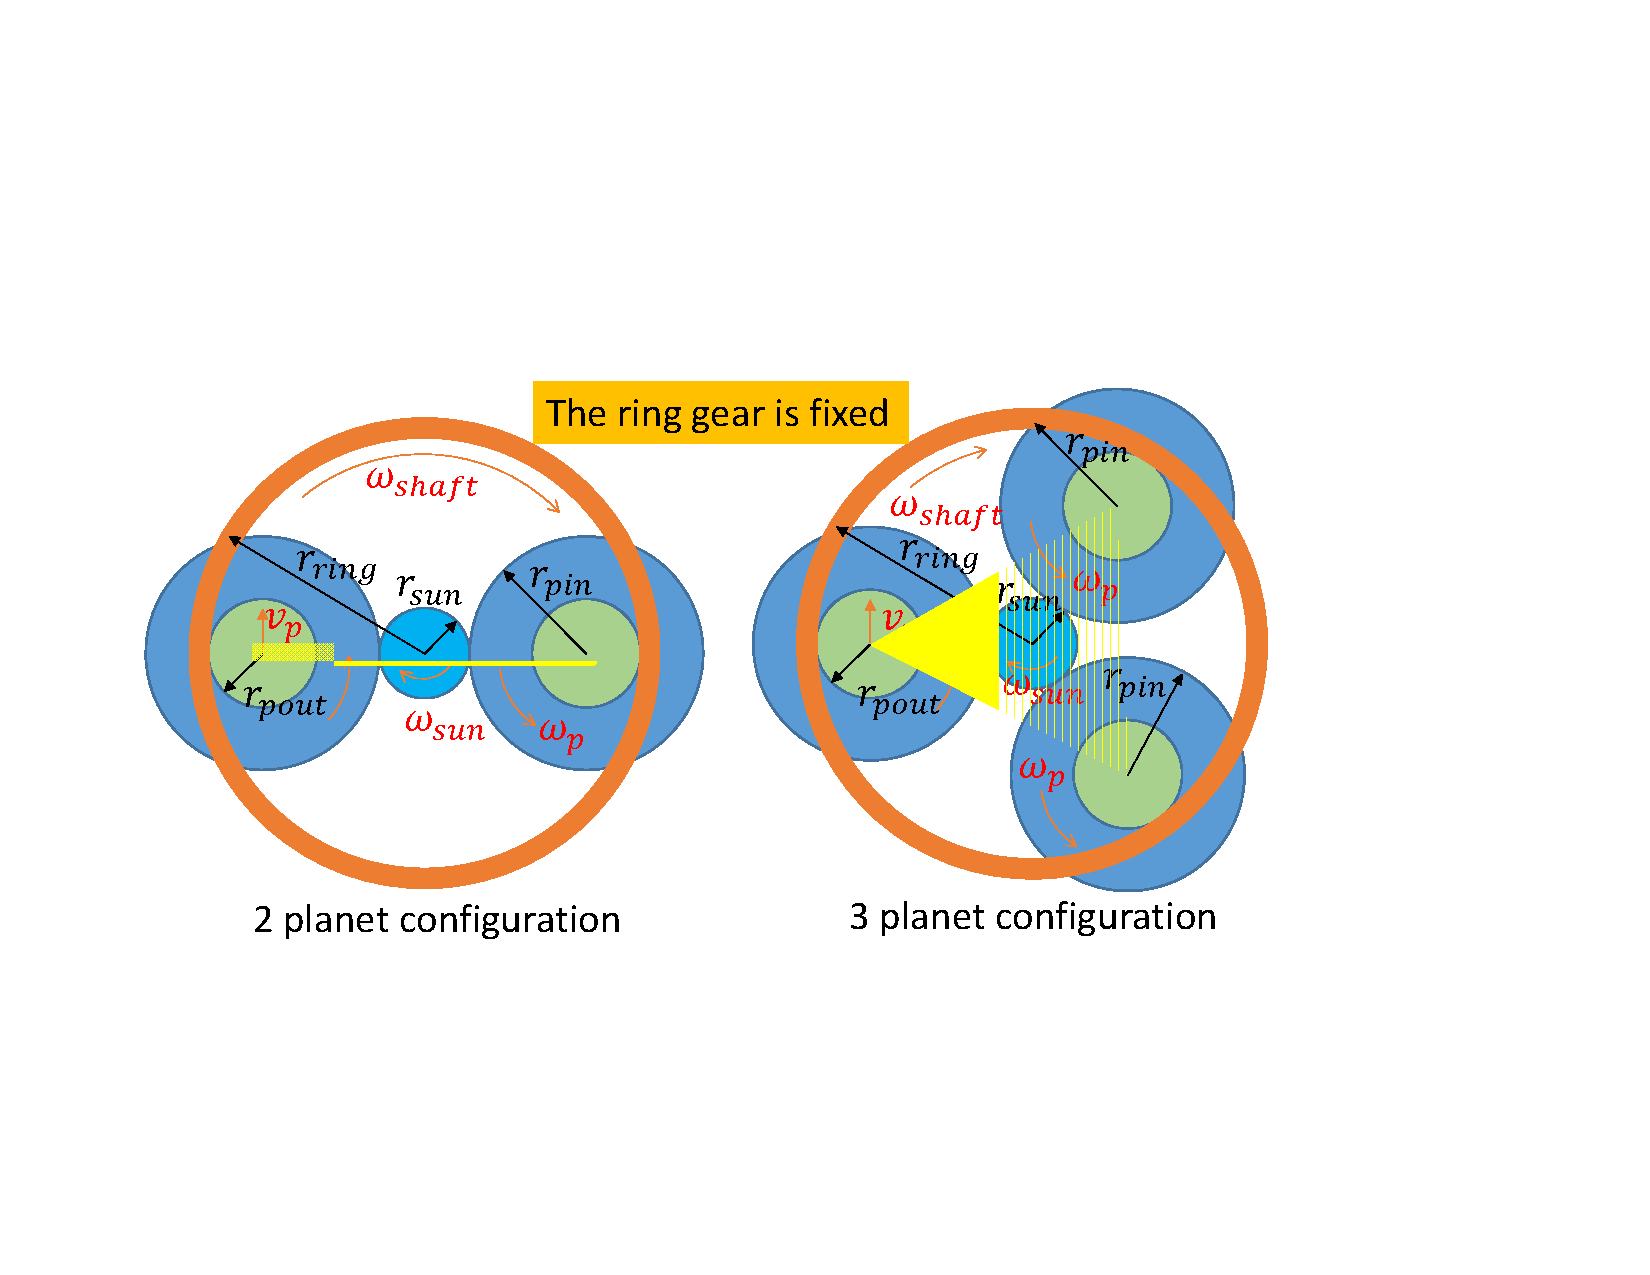
\includegraphics{planetaryGearbox.pdf}}
	\caption{Schematics of Compound Planetary Gearbox Configurations. (left) 2 planet configuration, (right) 3 planet configuration}
	\label{fig:planetaryGearbox}
\end{figure}

The objective of compound planetary gearbox design is to achieve desired gear ratio within dimensional constraints imposed by motor selection. In order to derive the gear ratio for given gear teeth number, a schematics of the two-stage compound planetary gearbox is used as shown in Figure \ref{fig:planetaryGearbox}. For given gear teeth numbers, both configurations in Figure \ref{fig:planetaryGearbox} are equivalent. Some assumptions for this analysis is posed here: 

\begin{enumerate}
	\item The sun gear located at the center is the input.
	\item The output shaft shown as yellow transparent shape is the output.
	\item The output shaft is connected to the axes of all the planet gears.
	\item The sun gear is meshed with input planet gears.
	\item The ring gear is meshed with output planet gears.
	\item The ring gear is fixed.
\end{enumerate}

Velocity equivalence is used to calculate the gear ratio.
\begin{eqnarray}
\omega_{sun} r_{sun} =& v_p + \omega_p r_{pin}\\
v_p =& \omega_{p} r_{pout}\\
\omega_p =& \frac{\omega_{sun}r_{sun}}{r_{pout}+r_{pin}}\\
\omega_{shaft} =& \frac{\omega_{p}r_{pout}}{r_{sun}+r_{pin}}
\end{eqnarray}
where $\omega_{shaft}$ is the angular velocity of the output shaft and the rest of the variable definitions could be found in Table \ref{tab:varDefGearbox}.

Therefore, the gear ratio of a compound planetary gearbox could be formulated as:
\begin{equation}
GR = \frac{\omega_{sun}}{\omega_{shaft}} = \frac{(r_{pout}+r_{pin})(r_{sun}+r_{pin})}{r_{sun}r_{pout}} = \frac{(N_{pout}+N_{pin})(N_{sun}+N_{pin})}{N_{sun}N_{pout}}
\end{equation}

\begin{table}[bp]
	\centering
	\caption{Variable Definition for Gear Ratio Calculation}
	\begin{tabular}{lcccc}\hline\hline
		& Sun gear		& Input planet	& Output planet	& Ring gear \\ \hline
		Pitch diameter	& $r_{sun}$	   	& $r_{pin}$		& $r_{pout}$	& $r_{ring}$\\
		Angular velocity& $\omega_{sun}$& $\omega_{p}$	& $\omega_{p}$	& N/A		\\
		Linear velocity	& N/A			& $v_p$			& $v_p$			& N/A		\\
		Teeth number	& $N_{sun}$		& $N_{pout}$	& $N_{pout}$	& $N_{ring}$\\ \hline
	\end{tabular}
	\label{tab:varDefGearbox}
\end{table}

The planetary gearbox shown in Figure \ref{fig:gearbox} utilizes two-stage compound planet gears to provide desired gear ratio while satisfying the dimensional constraints imposed by motor selection. 

The constraints for choosing teeth numbers are listed as follows:

\begin{enumerate}
	\item The teeth number of sun gear ($N_{sun}$) and ring gear ($N_{ring}$) could both be divided by the number of planet gears.
	\item The pitch circles of sun gear and planet gears, as well as that of planet gears and the ring gear should be externally tangent, 
	
	i.e. $r_{ring}=r_{sun}+r_{pin}+r_{pout}$ or $N_{ring}=N_{sun}+N_{pin}+N_{pout}$.
	\item The gear ratio $GR$ should be within the range of 22 - 25.
	\item The radius of the gearbox should be less than 25 mm, 
	
	i.e. $Max[r_{ring},r_{sun}+2r_{pin}]<12.5 mm$
	\item The teeth number for sun gear $N_{sun}$ should be no less than 6. Other wise the meshing would be problematic because the profile of gear teeth would be distorted too much.
\end{enumerate}

On top of the constraints, some practical issues were also considered in choosing gear teeth. Ideally, the phase difference between two stages of the planet gears should be the same. However, in compound gear manufacturing, the phase differnce could not be well maintained. To solve this problem, the planet gear teeth combination was chosen to be 16/53, which only share the common factor of 1. This choice provides tunable backlash with $2.1^{\circ}$ increment in the gearbox assembly. This is very similar to the working principle of a mechanical caliper, which uses two scales (main scale and vernier scale) with small difference to achieve high precision.

A large number of teeth combinations were enumerated taking into account all the constraints. The optimal gear teeth choice emerged as $N_{sun} = 12; N_{pin} = 53; N_{pout} = 16; N_{ring} = 81$ and the gear ratio is 23.3594.

All gears are custom made by \textit{HPC Gears Ltd} with 0.4 pitch and pressure angle of $20^{\circ}$.

%%%%%%%%%%%%%%%%%%%%%%%%%%%%%%%%%%%%%%%%
%          Leg Topology Comparison
%%%%%%%%%%%%%%%%%%%%%%%%%%%%%%%%%%%%%%%%
\section{Leg Topology Comparison}
\label{sec:LegComparison}
The full leg module will have three degrees of freedom (DOF) in order to achieve agile 3D maneuver. Three leg topologies, namely, open-serial chain, parallel five-bar and symmetric five-bar are analyzed in terms of workspace, force production and proprioceptive sensing. For simplicity, the abduction/adduction (ABAD) DOF is neglected and only motion in the 2-D hip-knee plane is analyzed. The analysis is based on the linkage analysis of Minitaur\cite{Kenneally2016}, but extended its analysis to negative $\delta$ value. Also, radial and lateral force, velocity and proprioceptive sensitivity are the three main concern in this section. In this section, all the analysis is based on the assumption of massless links, that is, no linkage mass or inertia is considered. This is valid in real application because the majority of mass is taken by actuators, which could be placed at the base of the link and transmit power via some kind of power transmission system like linkage, chain or belt. Therefore, linkage mass is relatively light compared to the body or even less than 10\% of the total mass, as shown in the MIT Cheetah design\cite{Hae-WonPark1PatrickM.Wensing22015}.

\begin{figure}
	\centering
	\resizebox{0.8\linewidth}{!}{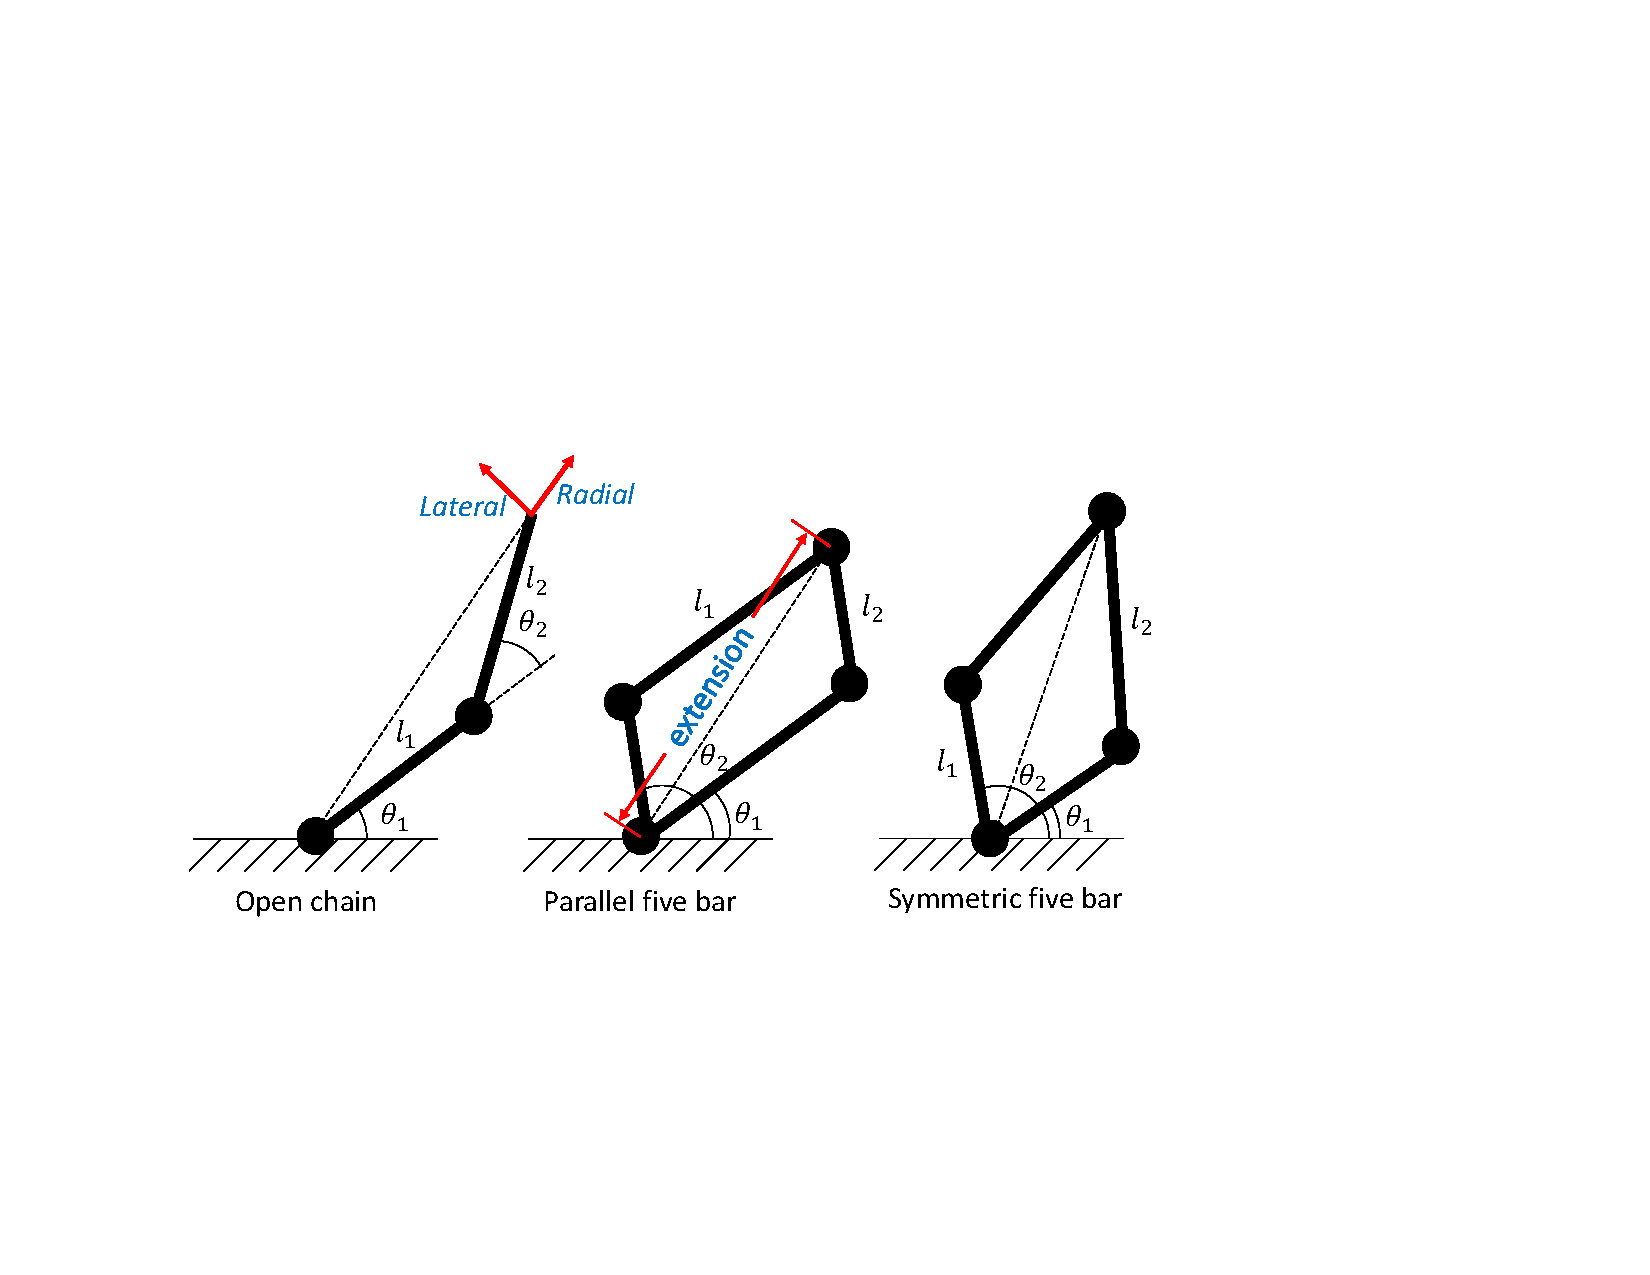
\includegraphics{linkages.pdf}}
	\caption{Three typical linkage topologies (a)Open-serial chain (b)Parallel five-bar (c)Symmetric five-bar. The design variable is $\delta$ and the workspace variable is the leg's radial extension}
	\label{fig:linkages}
\end{figure}

%-------------------------------------------
% ----------Workspace----------
\subsection{Workspace}
\label{sec:workspace}
 	For the three candidate leg topologies shown in Figure \ref{fig:linkages}, the workspace is an annulus, which could be characterized by maximum radius $r_{max}$ and minimum radius $r_{min}$ of the annulus. The design space is defined as:
 	\begin{equation}
 		\delta=\frac{r_{min}}{r_{max}}
 	\end{equation}
 	where $r_{max} = l_1 + l_2$ and $r_{min} = l_1 - l_2$, and $l_1,~l_2$ are the lengths of the first and second links shown in Figure \ref{fig:linkages}. Notice that here $\delta \in (-1,1)$, which means $l_1$ chould be either longer or shorter than $l_2$, which serves as an extension to the analysis presented in \cite{Kenneally2016}.
 	
%-------------------------------------------
% ----------Sweep Volume----------
\subsection{Sweep Volume}
\label{sec:sweepVolume}
	For quadrupedal robot application, sweep volume is also another important factor to consider in linkage design. Large sweep volume is not desirable because the four limbs of a quadrupedal robot are close to each other and the workspace would be decreased if the sweep volume is large. In addition, when interacting with unstructured terrain, large sweep volume increases the possibility of tripping and colliding. For example, when a robot is climbing upstairs, the leg sweep volume should stay clear of the stairs to avoid collision. In out door environment where there are debris and fabric that could easily tangle the robot, a slimmer and compact leg design would be more advantageous. Hence minimized sweep volume is favorable for quadrupedal robot leg design.

%-------------------------------------------
% ----------Force Production----------
\subsection{Force Production}
\label{sec:forceProduction}

	Manipulability ellipsoids are used to characterize a robot arm's ability to move in certain configuration\cite{Lynch2016}. In the following sections, manipulability ellipsoids of force production, velocity production and proprioceptive sensitivity are utilized to present a manipulator's mechanical performance.
	
	Force production ellipsoid characterizes how unit joint torque from motors will reflect as end-effector forces. Solution to equation \ref{eq:force_production} forms the Force production ellipsoid. The major and minor axes of the force production ellipsoid represent the end-effector's strongest and weakest ability to produce force at the respective directions.

	\begin{equation}\label{eq:force_production}
		E_{force} := \{F | F^T J J^T F = ||\tau|| , ||\tau||=1\}
	\end{equation}

	Radial/Lateral force production is defined as the end-effector force in radial/lateral directions given unit joint torque input. Figure \ref{fig:force_openChain} \ref{fig:force_fiveBar} \ref{fig:force_symm} show how force production ability changes over $extension$ and $\delta$.
	
	
	\begin{figure*}
		\centering
		\resizebox{\linewidth}{!}{\includegraphics{egLink_force_ellip.pdf}}
		\caption{Force production in radial direction for an example linkage design of Open-chain, Parallel five-bar and Symmetric five-bar}
		\label{fig:egLink_force_ellip}
	\end{figure*}
	
	\begin{figure*}
		\centering
		\resizebox{0.7\linewidth}{!}{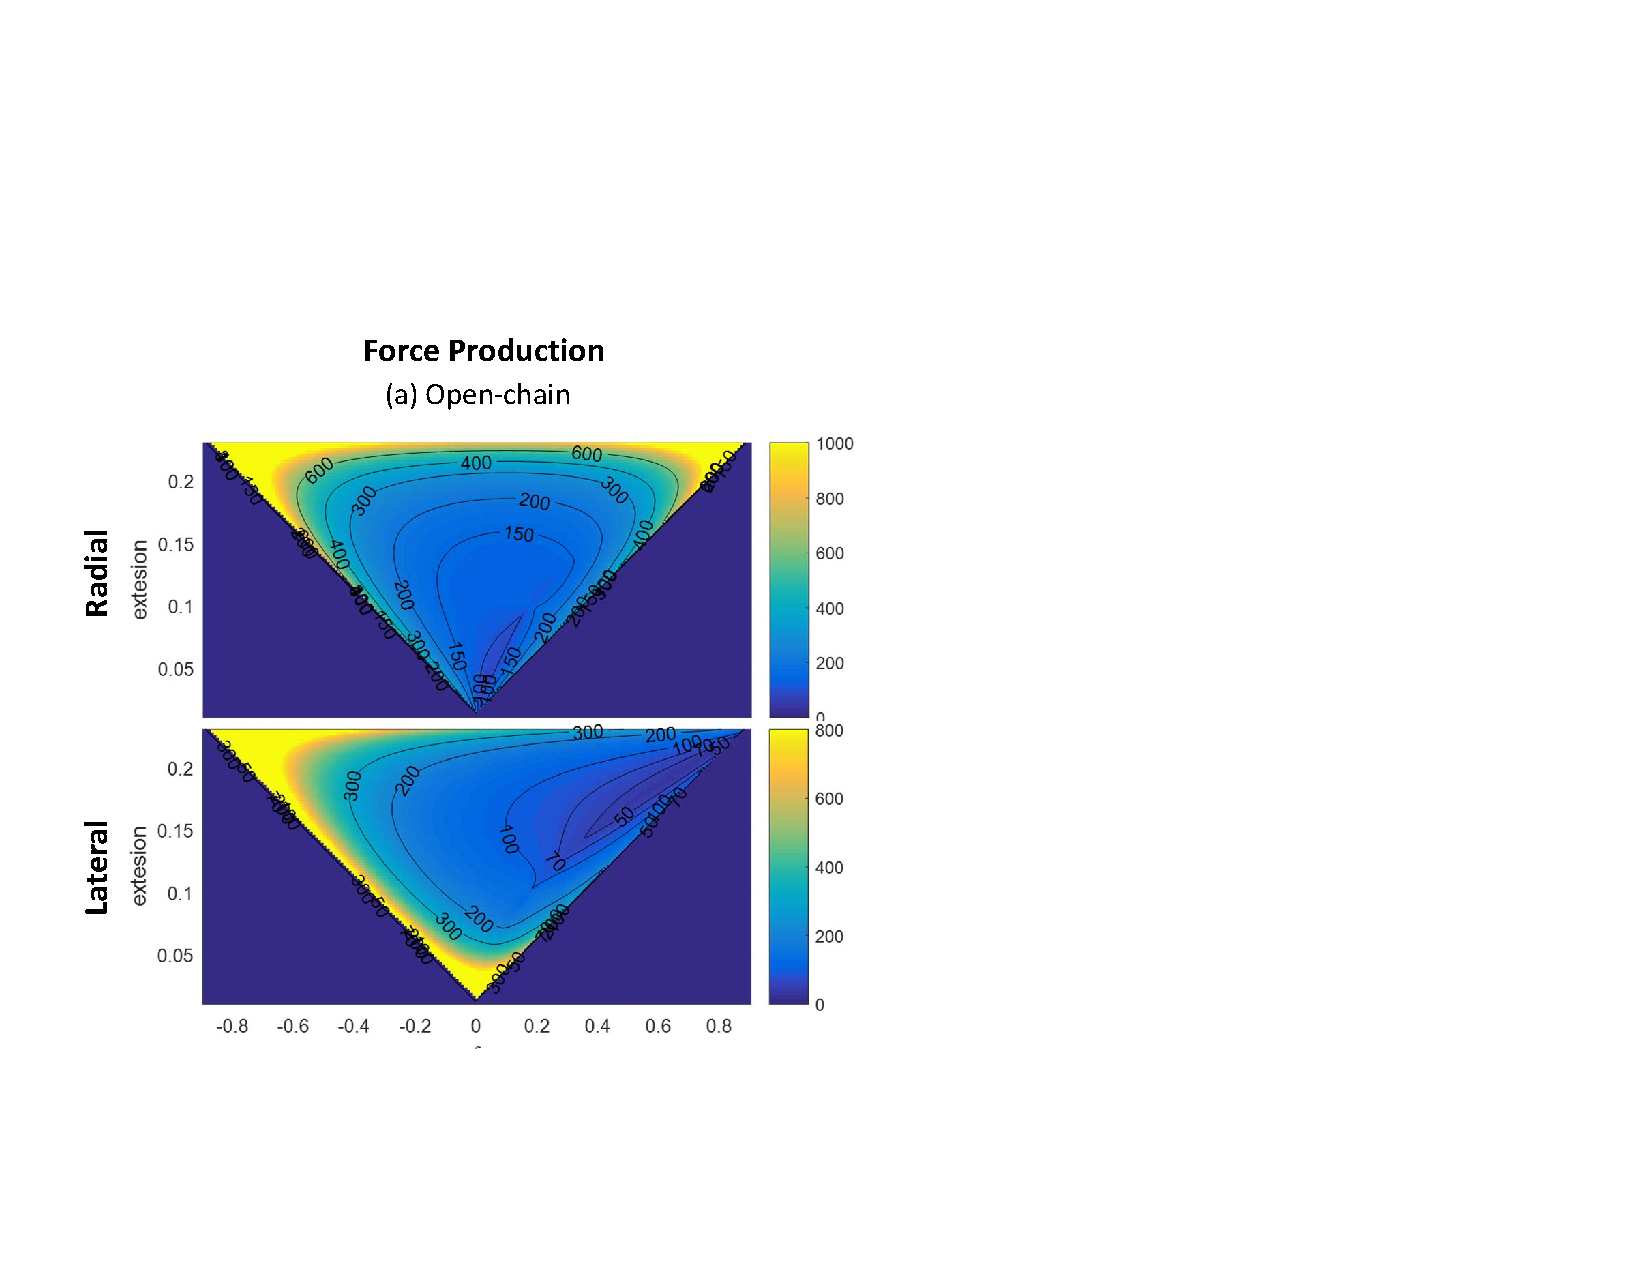
\includegraphics{force_openChain.pdf}}
		\caption{Force production in radial and lateral directions for open chain design}
		\label{fig:force_openChain}
	\end{figure*}

	\begin{figure*}
		\centering
		\resizebox{0.7\linewidth}{!}{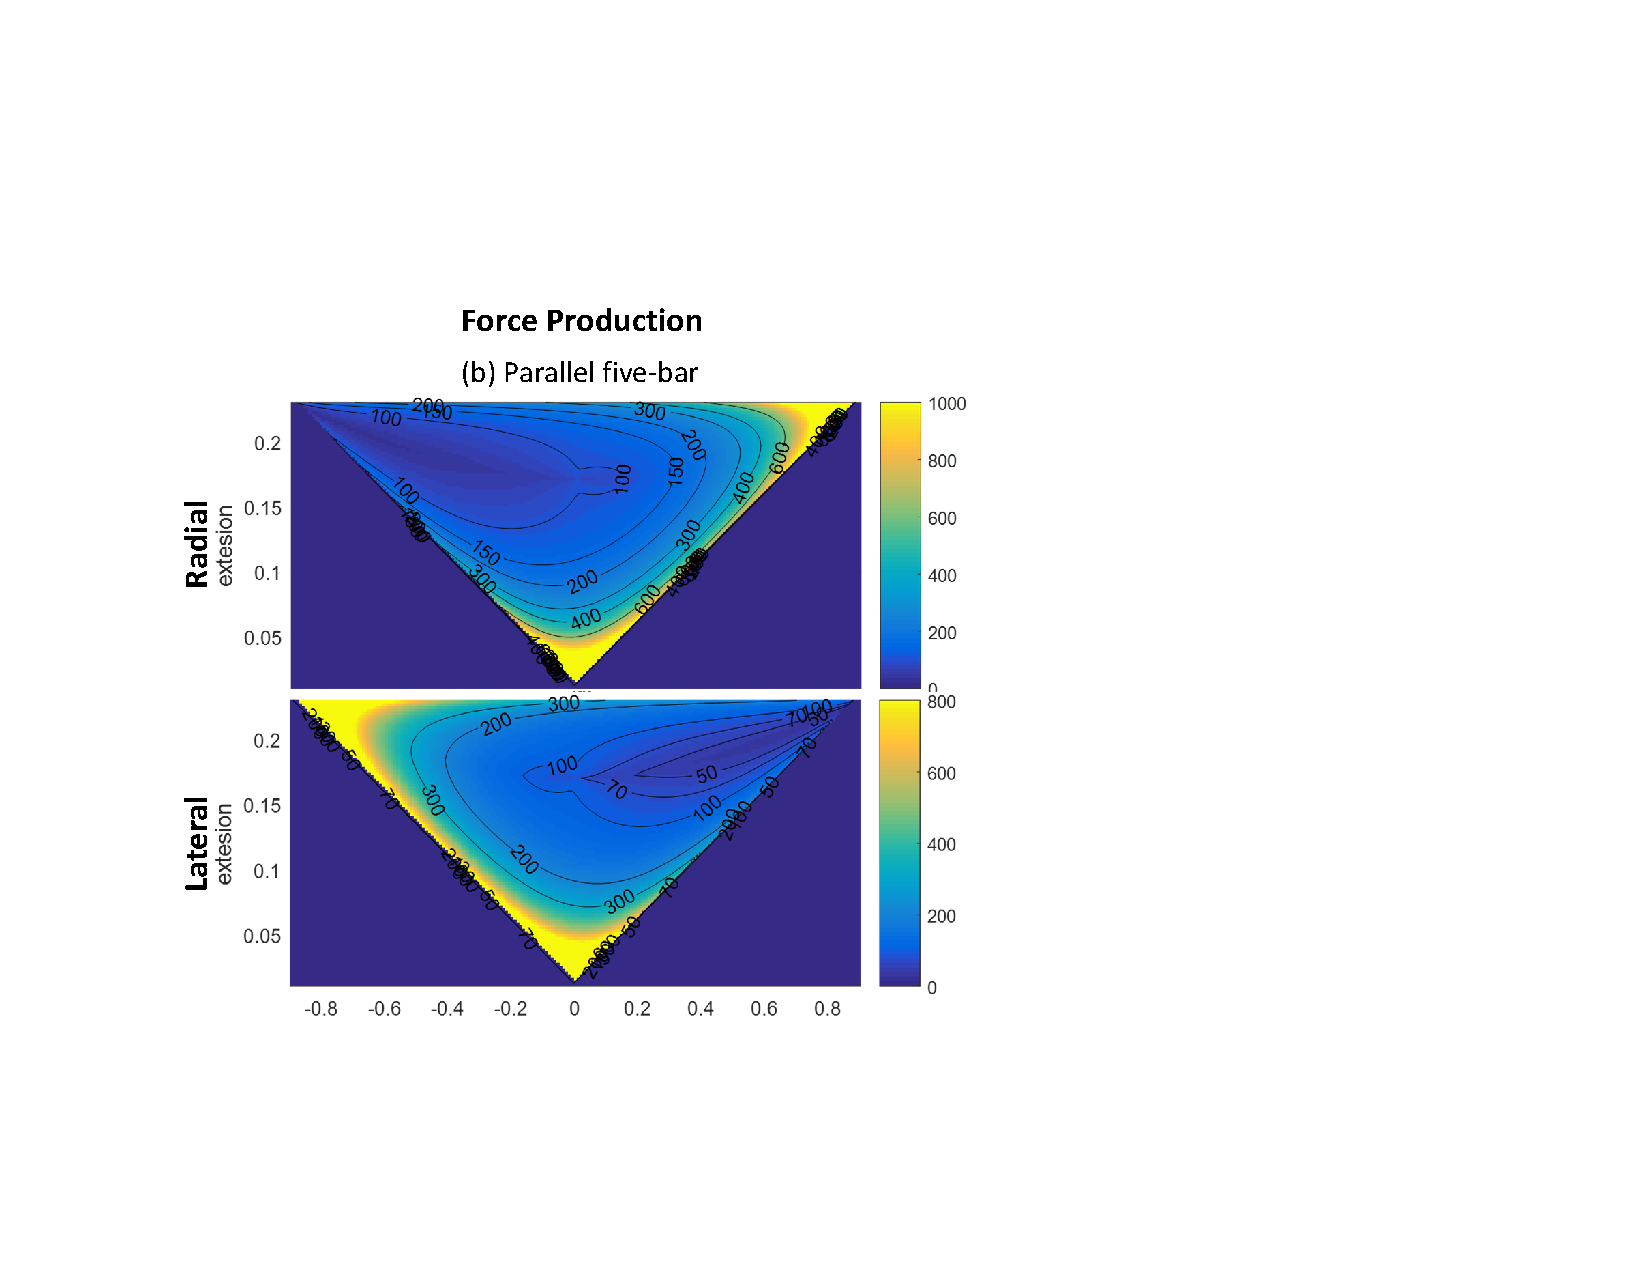
\includegraphics{force_fiveBar.pdf}}
		\caption{Force production in radial and lateral directions for parallel five-bar design}
		\label{fig:force_fiveBar}
	\end{figure*}

	\begin{figure*}
		\centering
		\resizebox{0.7\linewidth}{!}{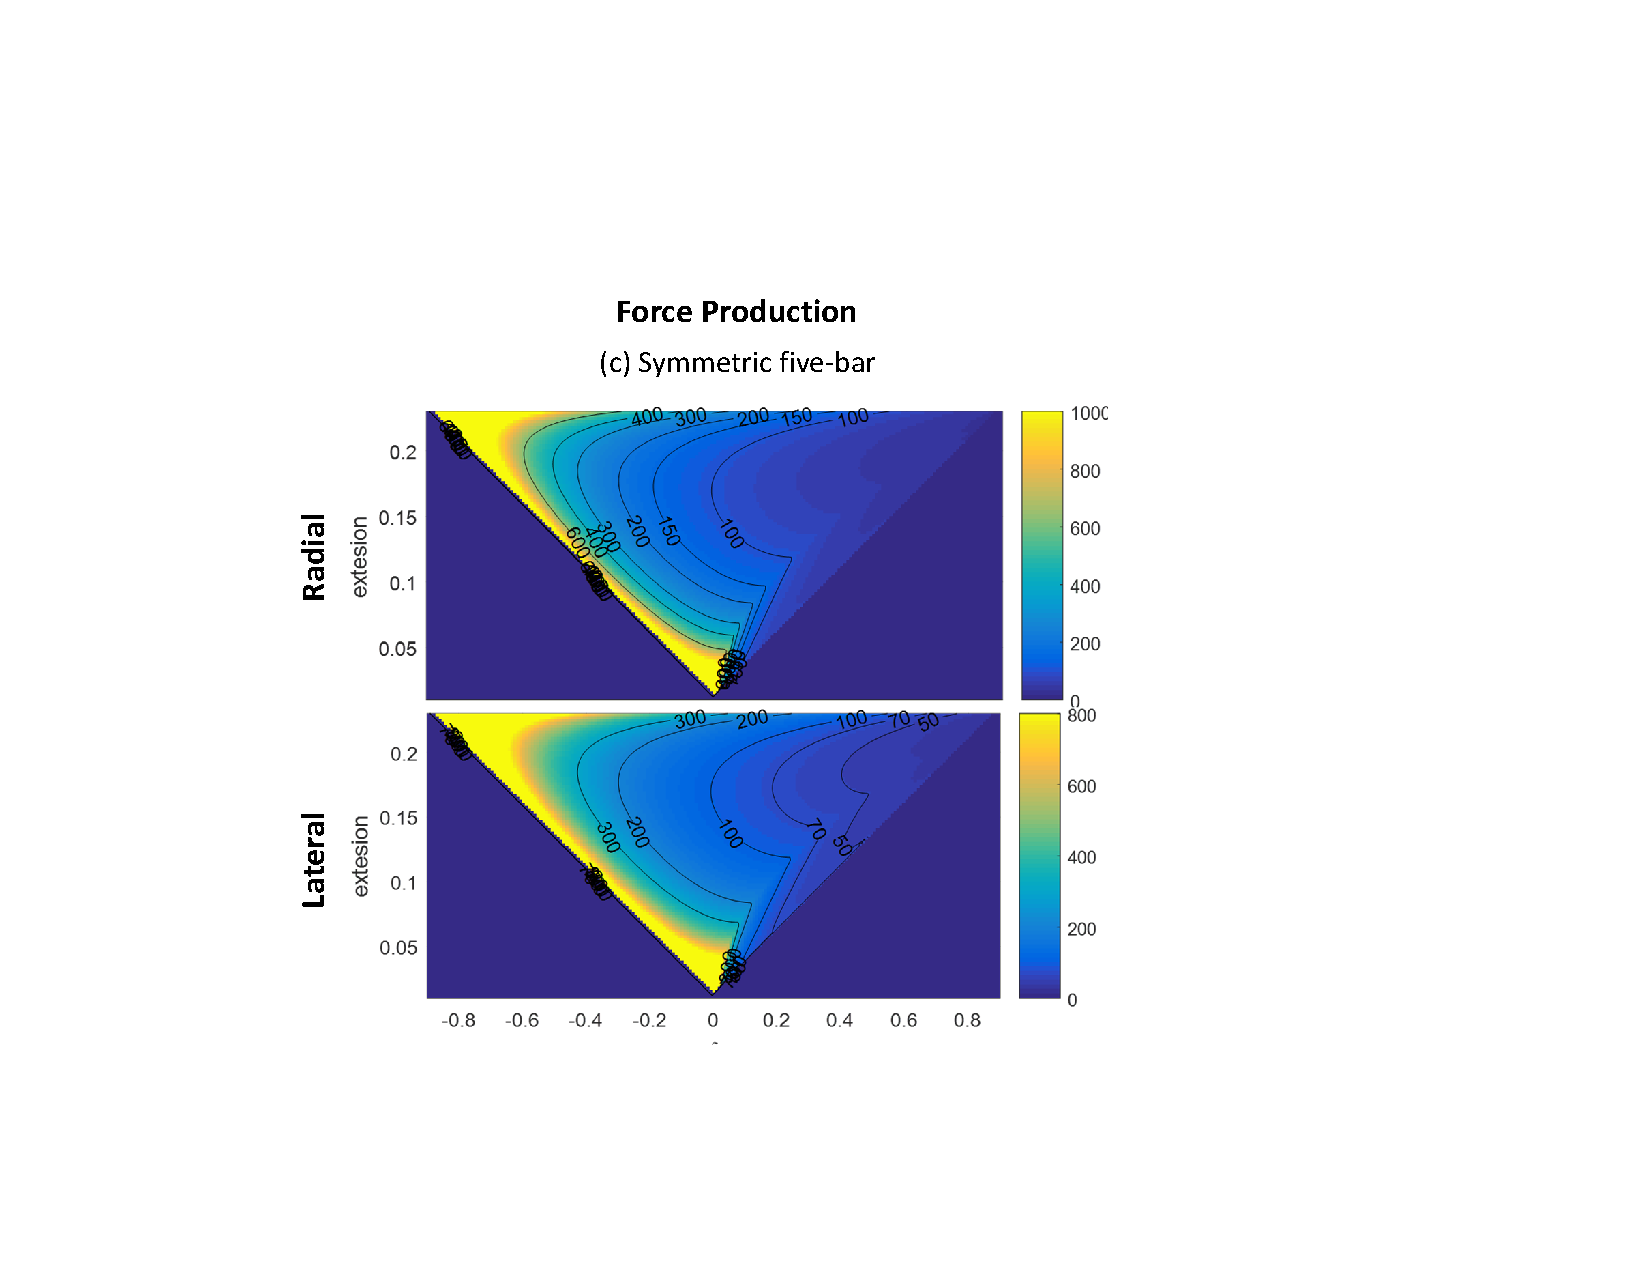
\includegraphics{force_symm.pdf}}
		\caption{Force production in radial and lateral directions for symmetric five-bar design}
		\label{fig:force_symm}
	\end{figure*}

%-------------------------------------------
% ----------Velocity Production----------
\subsection{Velocity Production}
\label{sec:velcotyProduction}

	\begin{figure*}
		\centering
		\resizebox{\linewidth}{!}{\includegraphics{egLink_vel_ellip.pdf}}
		\caption{Velocity production in radial direction for an example linkage design of Open-chain, Parallel five-bar and Symmetric five-bar}
		\label{fig:egLink_vel_ellipp}
	\end{figure*}

	\begin{figure*}
		\centering
		\resizebox{0.7\linewidth}{!}{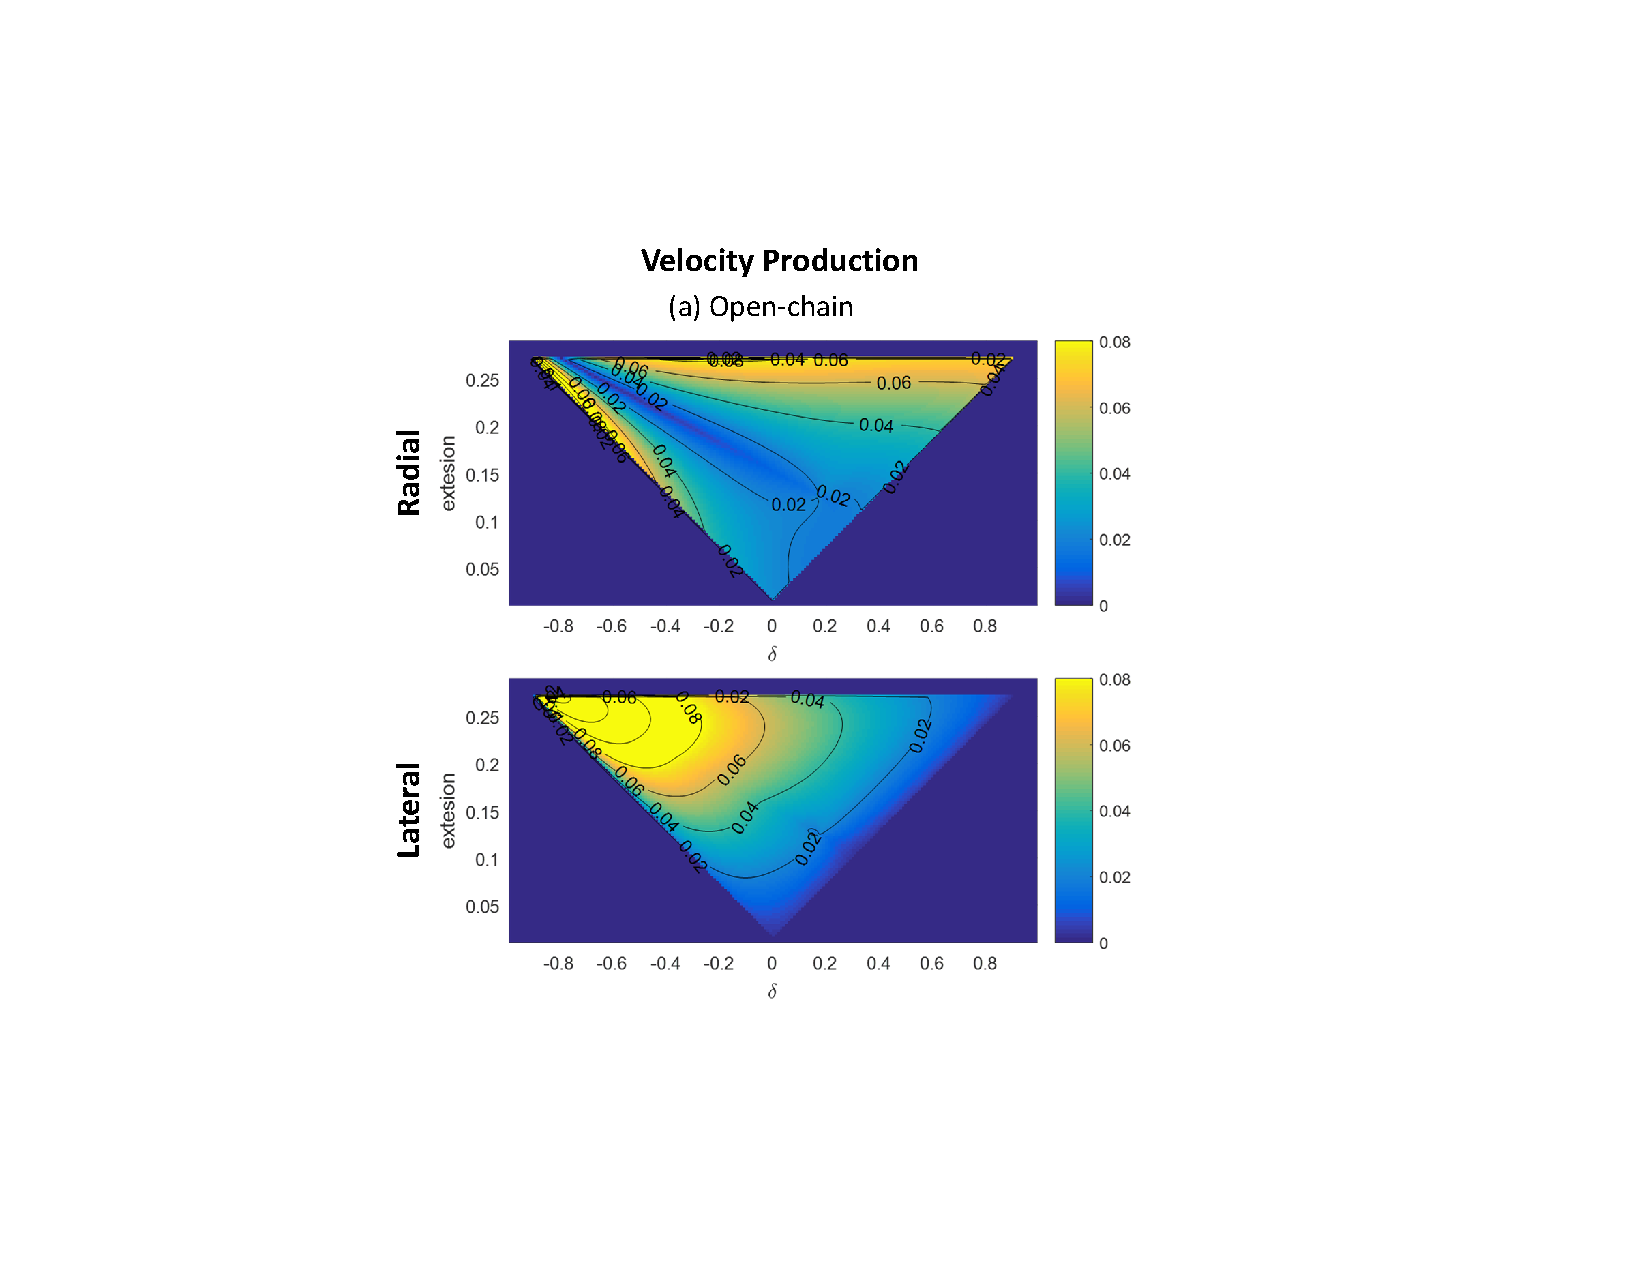
\includegraphics{vel_openChain.pdf}}
		\caption{Velocity production in radial and lateral directions for open chain design}
		\label{fig:vel_openChain}
	\end{figure*}
	
	\begin{figure*}
		\centering
		\resizebox{0.7\linewidth}{!}{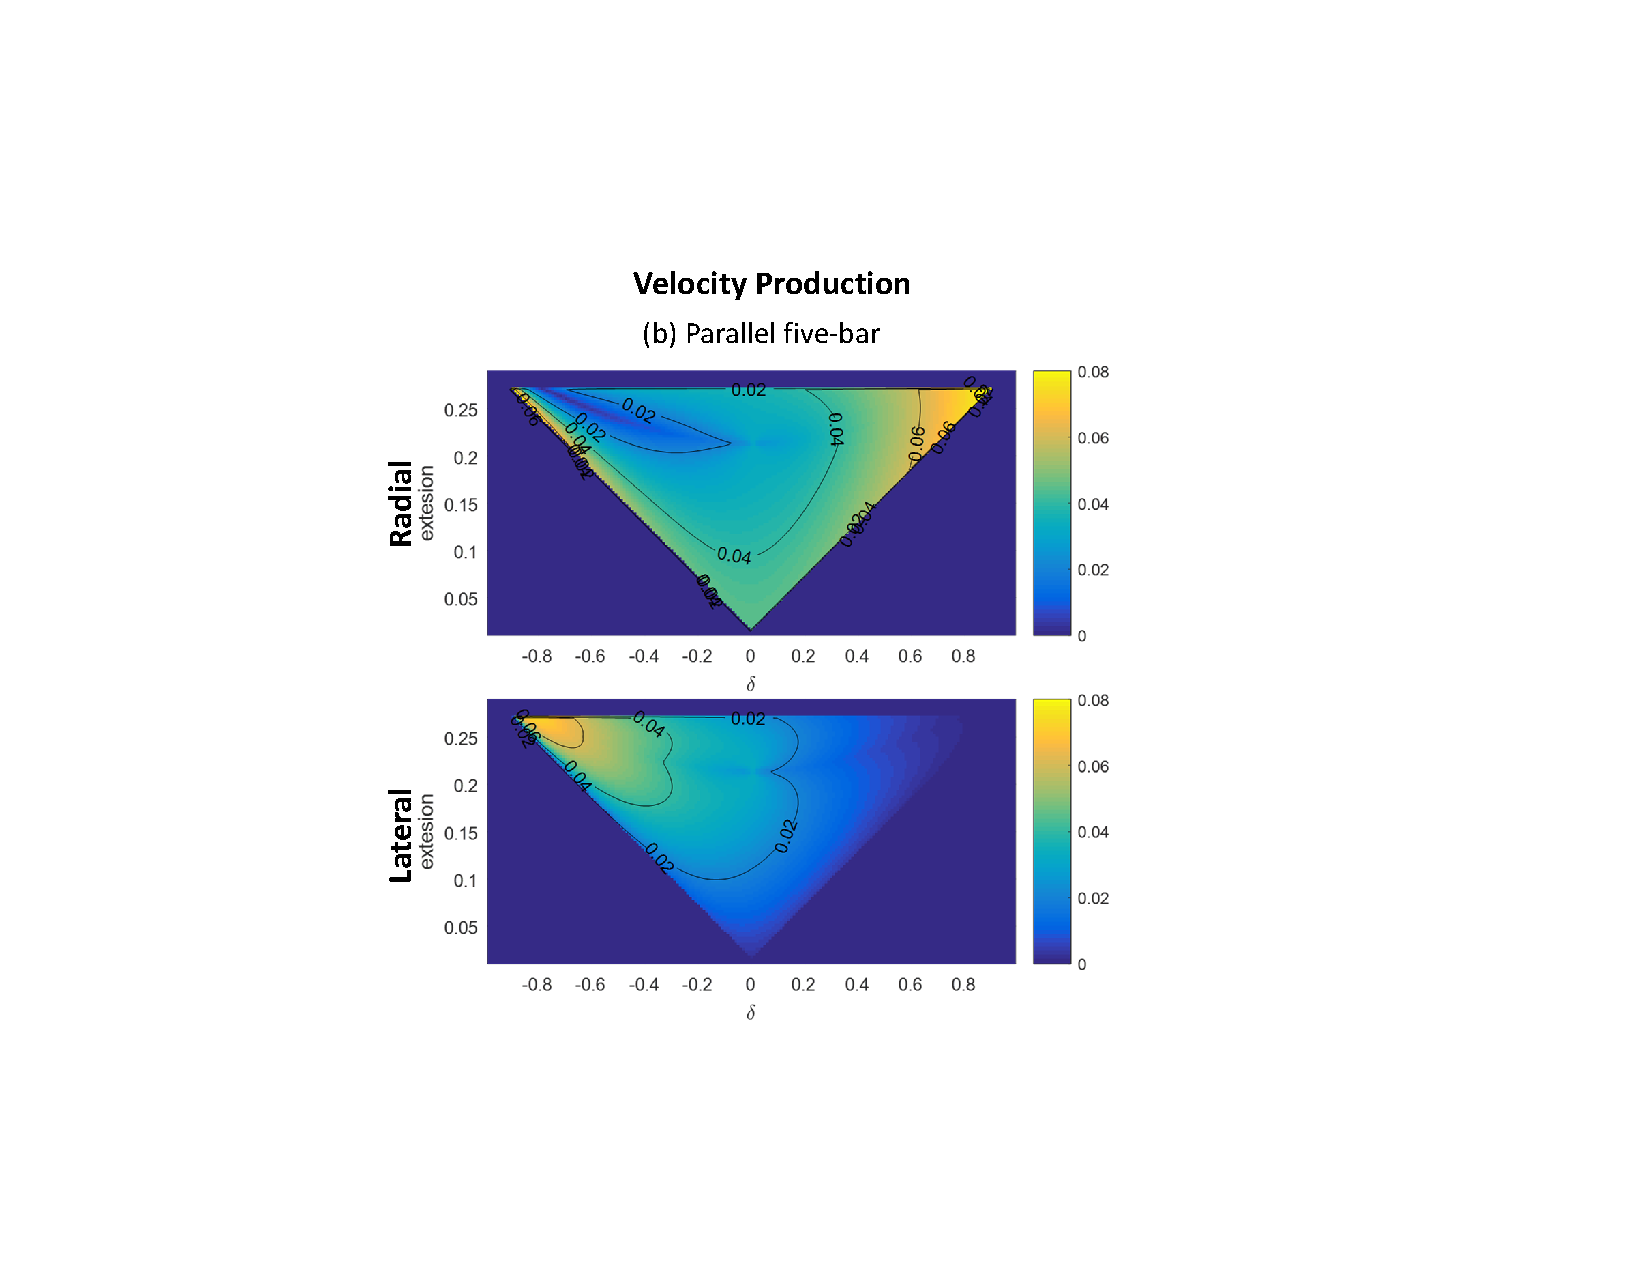
\includegraphics{vel_fiveBar.pdf}}
		\caption{Velocity production in radial and lateral directions for parallel five-bar design}
		\label{fig:vel_fiveBar}
	\end{figure*}
	
	\begin{figure*}
		\centering
		\resizebox{0.7\linewidth}{!}{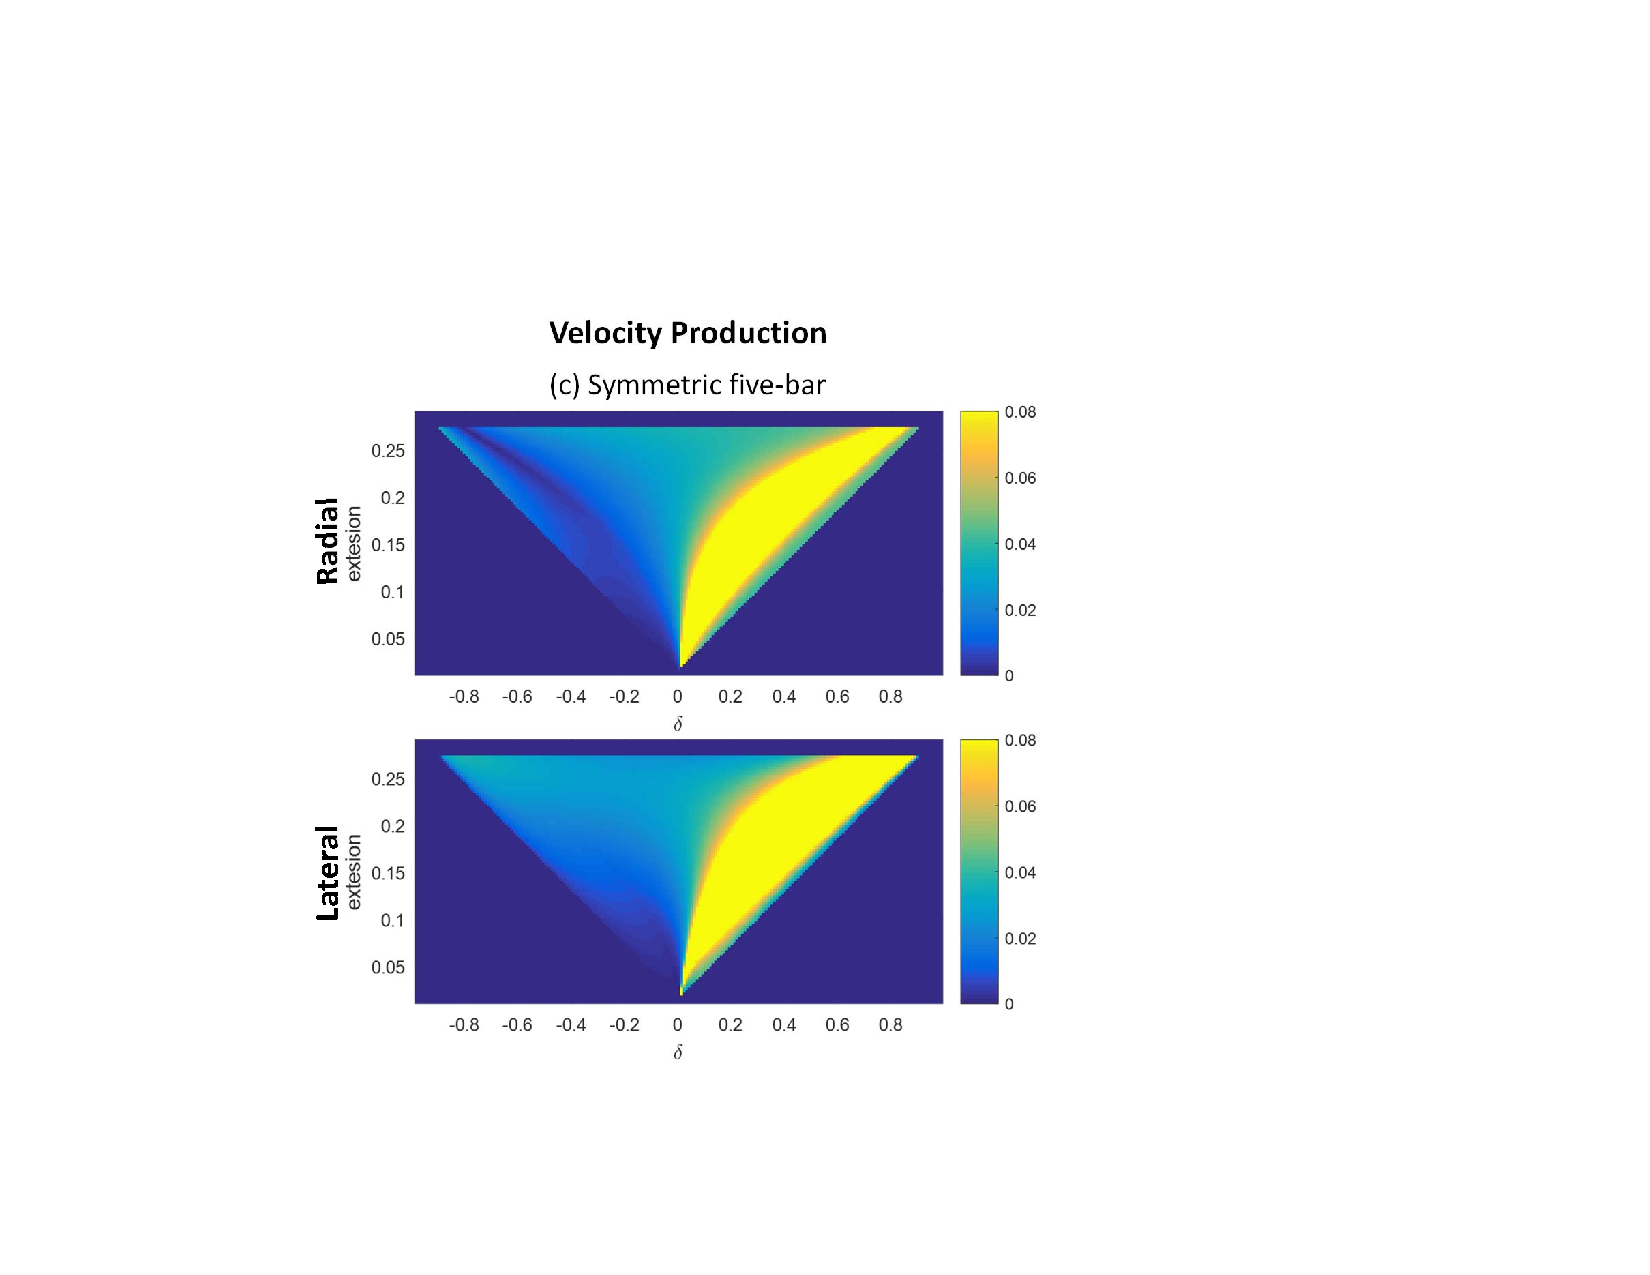
\includegraphics{vel_symm.pdf}}
		\caption{Velocity production in radial and lateral directions for symmetric five-bar design}
		\label{fig:vel_symm}
	\end{figure*}

	Velocity production ellipsoid characterizes how unit joint velocity from motors will reflect as end-effector velocity. Solution to equation \ref{eq:vel_production} forms the velocity production ellipsoid. The major and minor axes of the velocity production ellipsoid represent the end-effector's strongest and weakest ability to produce velocity at the respective directions.
	
	\begin{equation}\label{eq:vel_production}
		E_{velocity} := \{V | (J^{-1}v)^T(J^{-1}v)=||\omega|| , ||\omega||=1\}
	\end{equation}
	
	Radial/Lateral velocity production is defined as the end-effector velocity in radial/lateral directions given unit joint angular velocity input. Figure \ref{fig:force_openChain} \ref{fig:force_fiveBar} \ref{fig:force_symm} show how velocity production ability changes over $extension$ and $\delta$.


%-------------------------------------------
% ----------Proprioceptive Sensing----------
\subsection{Proprioceptive Sensing}
\label{sec:propSense}

	Proprioceptive sensitivity ellipsoid represents how unit force applied at the end-effector is visible to the motors. Solution to equation	 \ref{eq:sensitivity} forms the proprioceptive sensitivity ellipsoid.

	\begin{equation}\label{eq:sensitivity}
		E_{sensitivity} := \{\tau | \tau^T J^{-1}J^{-T}\tau = ||F||, ||F||=1\}
	\end{equation}
	
	\begin{figure*}
		\centering
		\resizebox{\linewidth}{!}{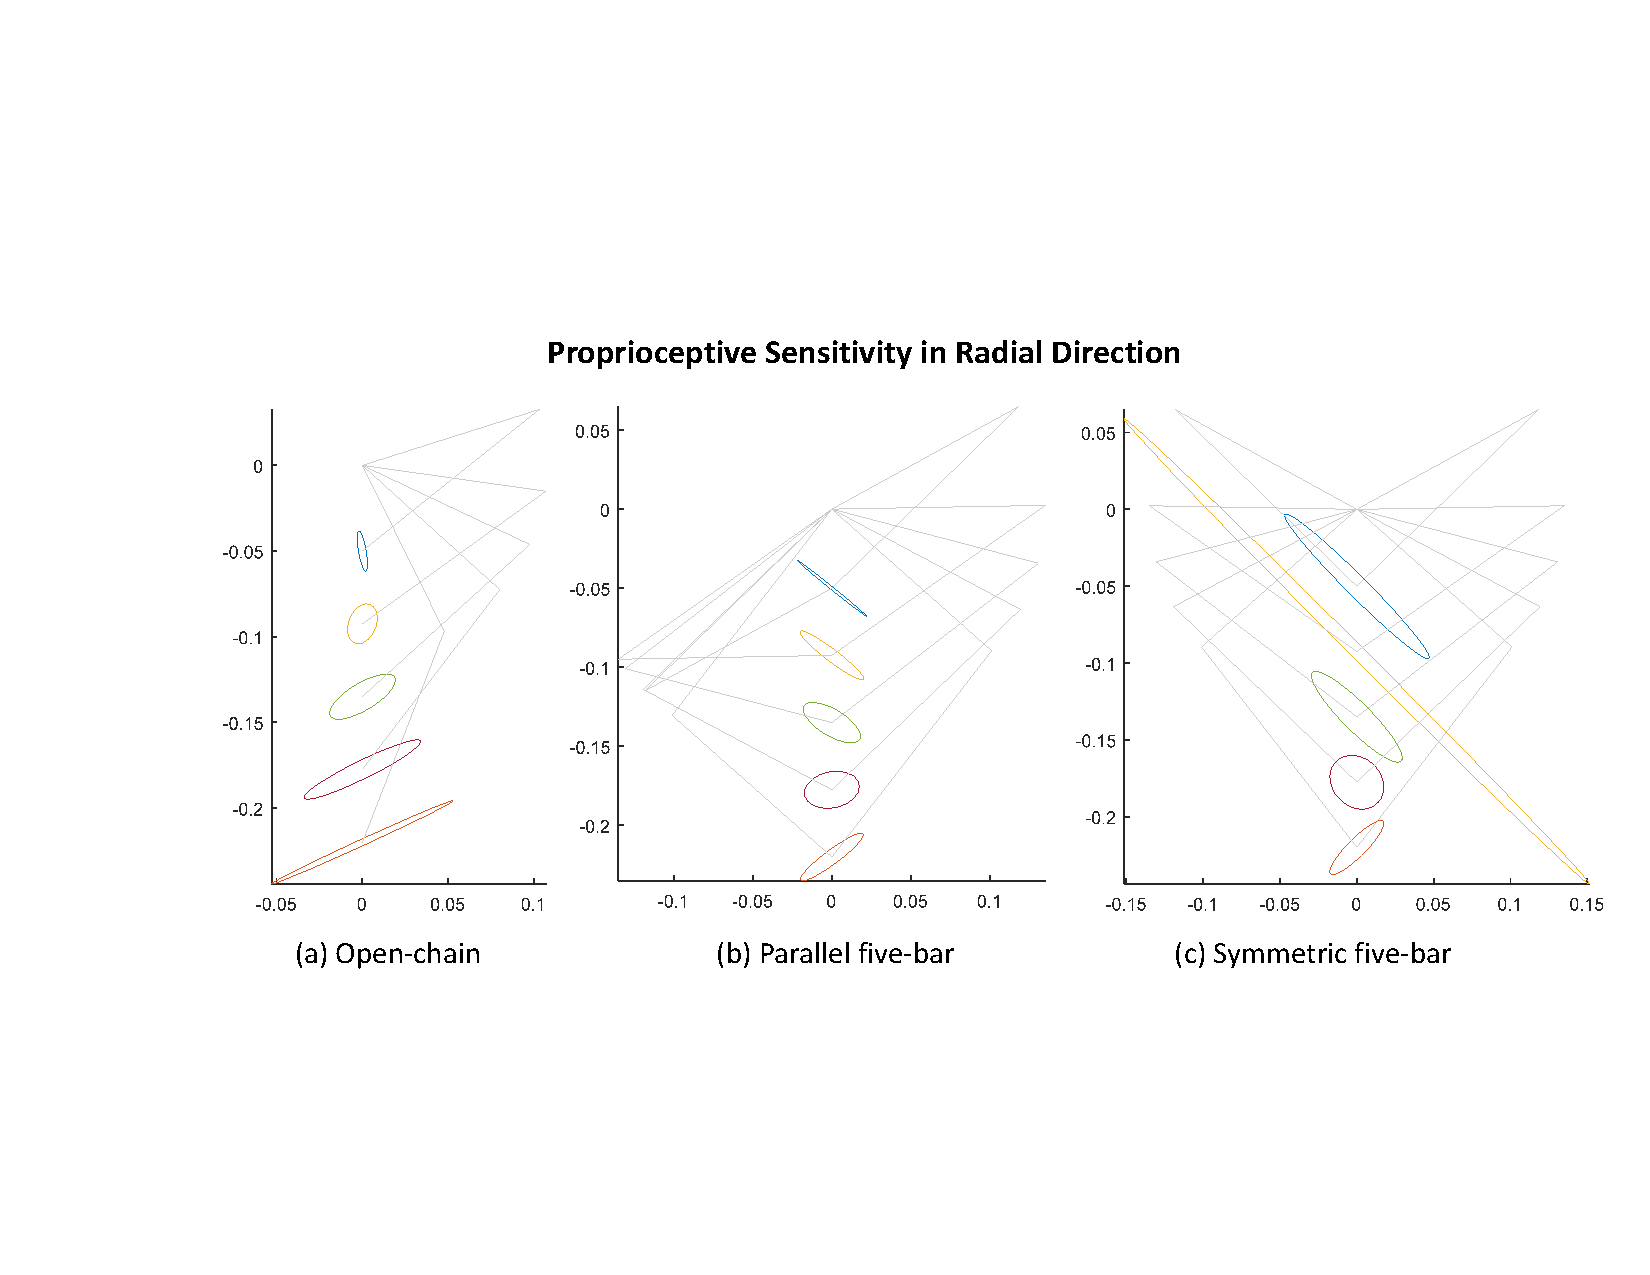
\includegraphics{egLink_sensi_Ellip.pdf}}
		\caption{Proprioceptive Sensitivity in radial direction for an example linkage design of Open-chain, Parallel five-bar and Symmetric five-bar}
		\label{fig:egLink_sensi_Ellip}
	\end{figure*}
	
	\begin{figure*}
		\centering
		\resizebox{0.7\linewidth}{!}{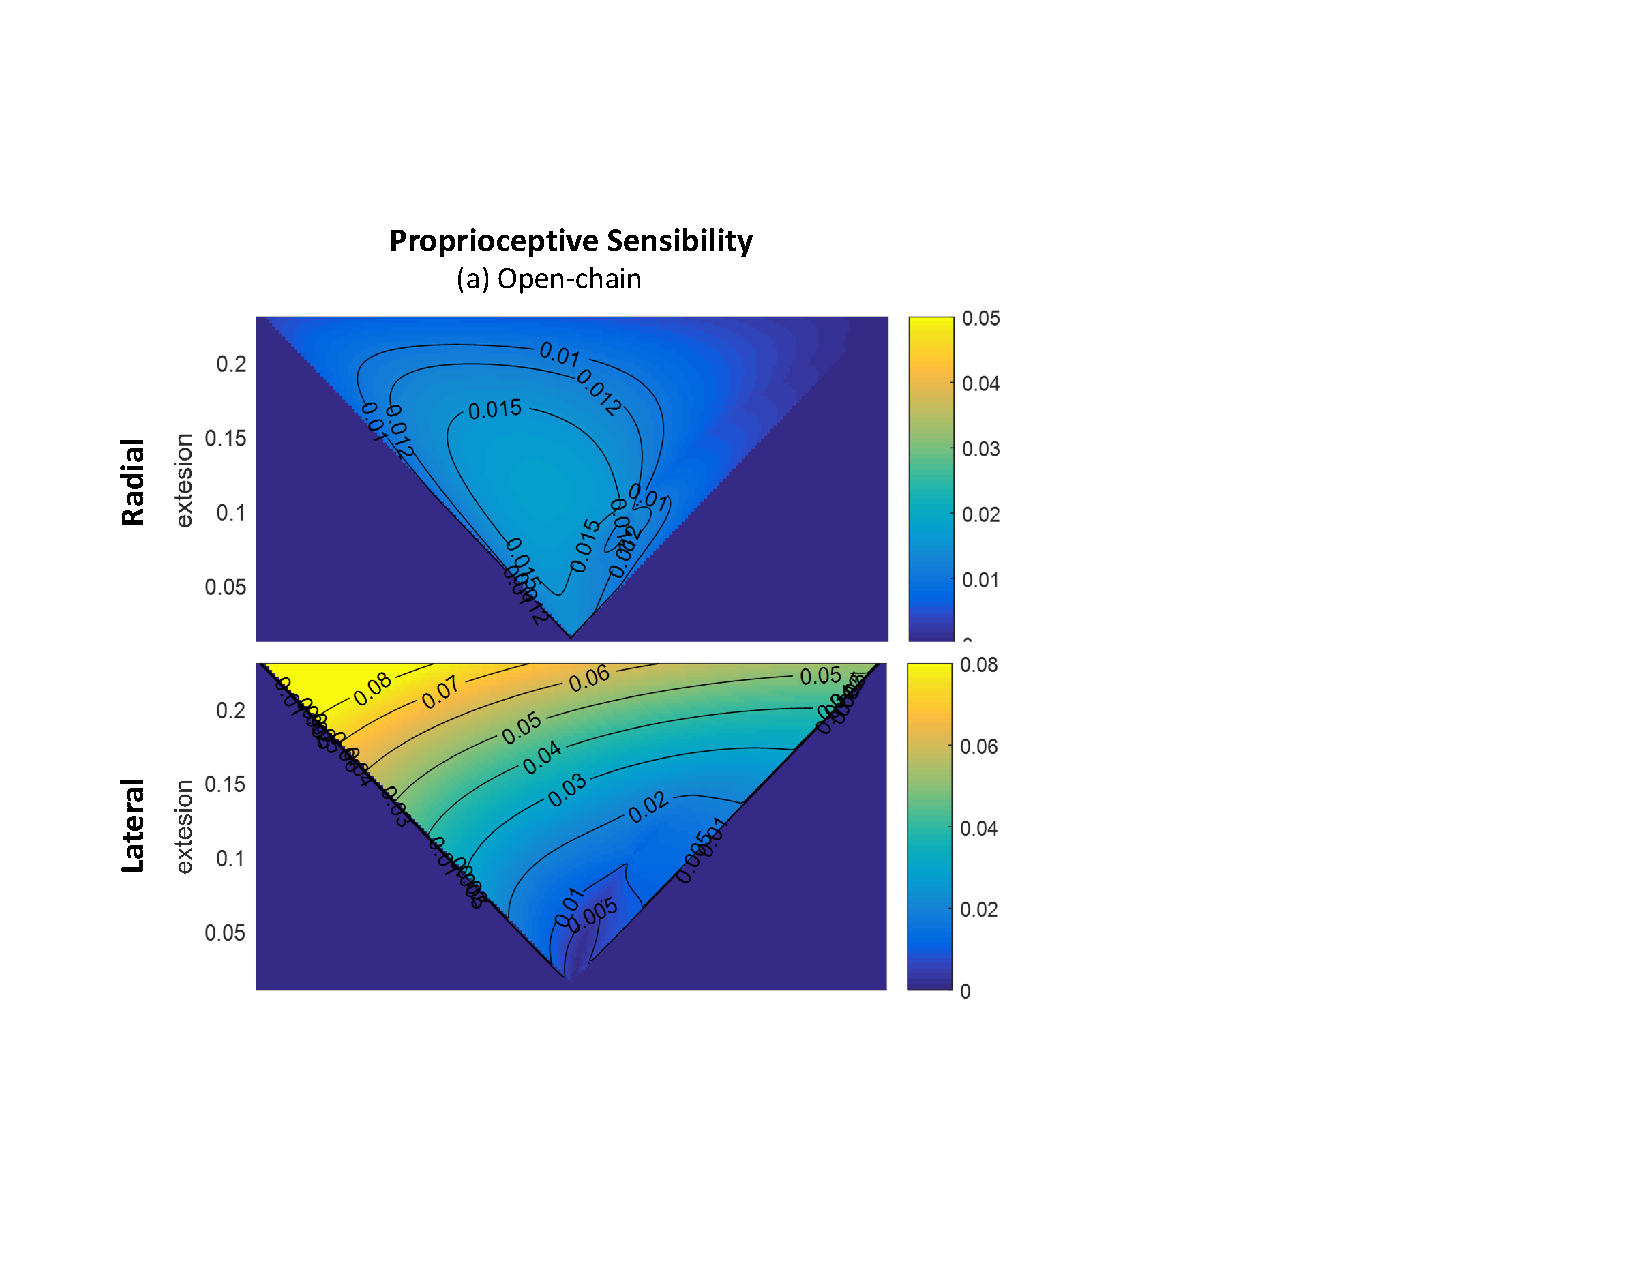
\includegraphics{sensitivity_openChain.pdf}}
		\caption{Proprioceptive Sensitivity in radial and lateral directions for the open-chain design}
		\label{fig:pro_sensitivity_openChain}
	\end{figure*}
	
	\begin{figure*}
		\centering
		\resizebox{0.7\linewidth}{!}{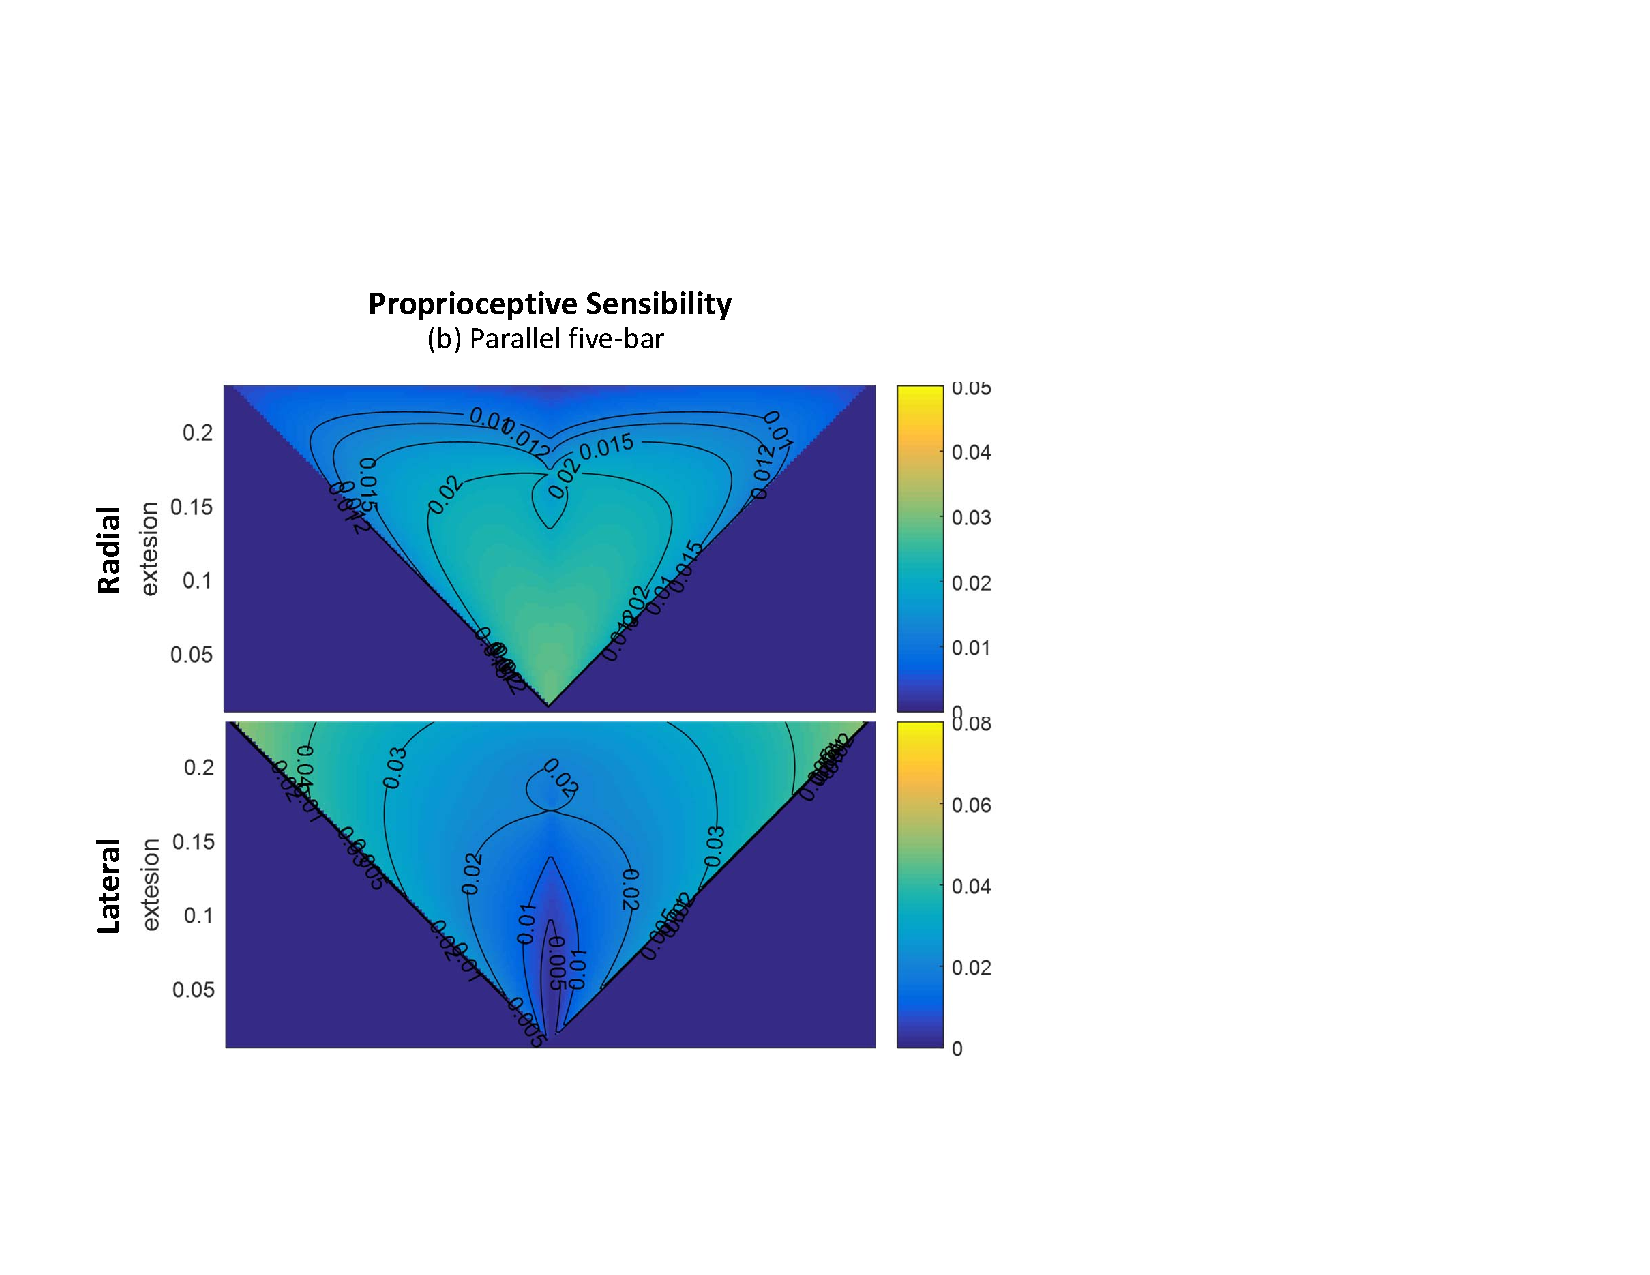
\includegraphics{sensitivity_fiveBar.pdf}}
		\caption{Proprioceptive Sensitivity in radial and lateral directions for the parallel five-bar design}
		\label{fig:pro_sensitivity_fiveBar}
	\end{figure*}
	
	\begin{figure*}
		\centering
		\resizebox{0.7\linewidth}{!}{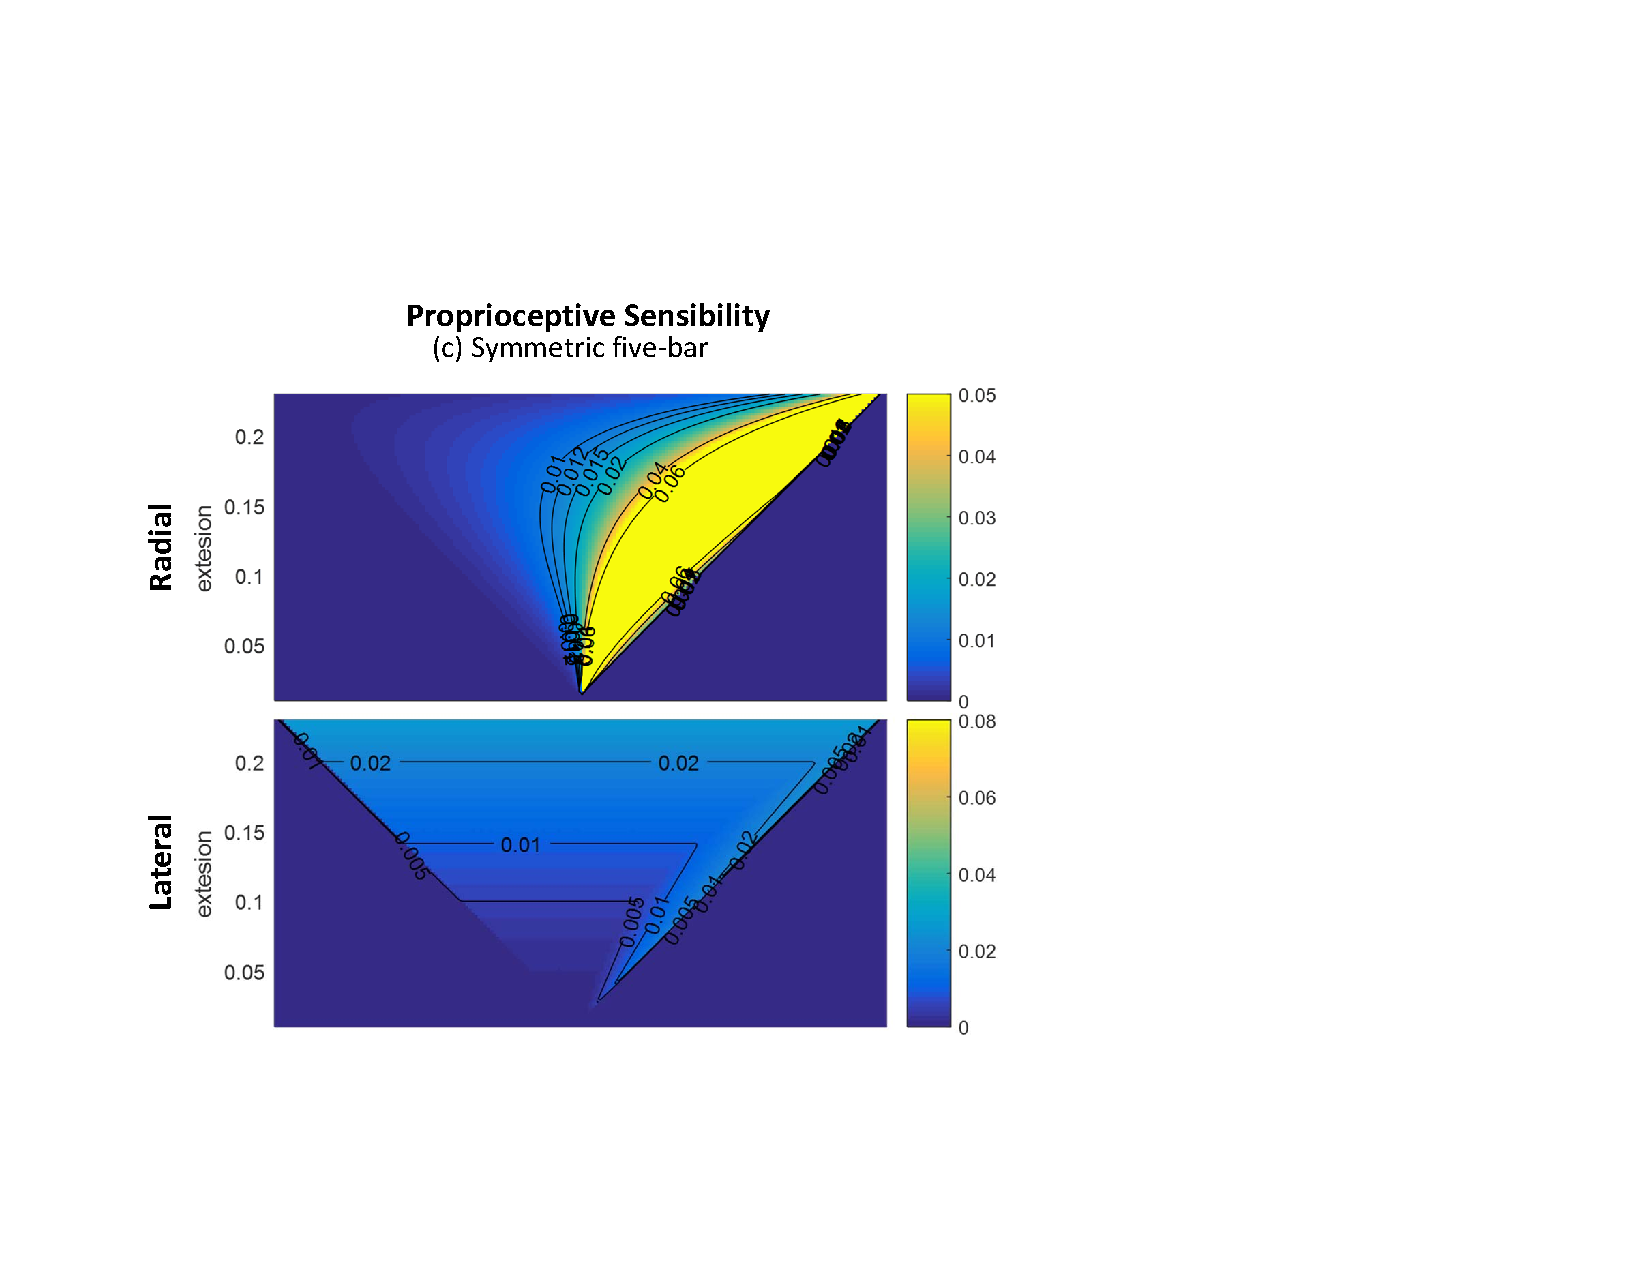
\includegraphics{sensitivity_symm.pdf}}
		\caption{Proprioceptive Sensitivity in radial and lateral directions for the symmetric five-bar design}
		\label{fig:pro_sensitivity_symm}
	\end{figure*}
	
	An example linkage design for the thee leg topologies is shown in Figure \ref{fig:egLink_sensi_Ellip} where design parameter $\delta$ is fixed as 0.1 and workspace parameter $extension$ is varied. The figure shows that in this specific example, the area enclosed by proprioceptive sensitivity ellipsoid is almost the same with symmetric five-bar slightly better.

	It is worth remarking that similar to force and velocity production, proprioceptive sensitivity should not only be considered in the radial direction, but also in the lateral direction. Radial/Lateral Proprioceptive Sensitivity is defined as the joint torque magnitude when radial/lateral unit force is applied at the end-effector. Figure \ref{fig:pro_sensitivity_openChain}, \ref{fig:pro_sensitivity_fiveBar}, \ref{fig:pro_sensitivity_symm} show how proprioceptive sensitivity changes over design parameters $extension$ and workspace variable $\delta$.
	
	Figure \ref{fig:pro_sensitivity_openChain}, \ref{fig:pro_sensitivity_fiveBar}, \ref{fig:pro_sensitivity_symm} show that while symmetric five-bar has excellent radial proprioceptive sensitivity, its lateral sensitivity is relatively poorer. In contrast, Open-chain design has better lateral proprioceptive sensitivity. Higher lateral sensitivity renders open-chain design advantageous in controlling horizontal forces, which is useful in applications such as jumping forward to precise location, control horizontal speed in running and so on.
	
	%-------------------------------------------
	% ----------Power Delivery----------
	\subsection{Power Delivery}
	\label{sec:powerDelivery}
	
	Since the velocity and force ellipsoids have their major axis coincide with the other's minor axis and vice versa, this means they are conjugate of each other. Thus the power delivery in every direction of the linkage design is assumed to be the same. But the manipulator analysis is static so only fixed instances are considered.
	
	
	%-------------------------------------------
	% ----------Linkage Design----------
	\subsection{Linkage Design}
	\label{sec:LinkageDesign}
	
	Although symmetric five-bar has excellent velocity production ability in both radial and lateral directions, its proprioceptive sensitivity in lateral direction is not very good. In addition, both parallel and symmetric five-bar design suffer from too large sweep volume, which is not desirable for quadrupedal robot locomotion, especially in unstructured terrain. Therefore, open-chain topology is chosen to be the linkage design.
	
	The previous sections have provided a recipe to come up with suitable link design for specific applications. An optimal design could be found by defining a cost function that pertains to application requirements. 
	
	\begin{equation}\label{eq:obj_func}
		Cost = - (w_{F_r} F_r + w_{F_l} F_l + w_{V_r} V_r + w_{V_l} V_l + w_{S_r} S_r + w_{S_r} S_r) + w_{\delta}\delta
	\end{equation}
	
	
	where $F_r,F_l,V_r,V_l,S_r,S_l$ are the force production and $\delta$ is as defined before, velocity production and proprioceptive sensitivity values in the radial and lateral directions, which is \textbf{normalized} by the average value in the span of $extension$ to get rid of the effect of magnitude of unit. $w_{F_r},w_{F_l},w_{V_r},w_{V_l},w_{S_r},w_{S_r},w_{\delta}$ are weighting factors that corresponds to the values. Higher weight could be put on the value that plays an important role on the application. For example, if a robot is designed to perform mostly in situations where high force production is required while operating in a low velocity region, the weighting factor for force production could be higher and the weighting factors for velocity production could be lower. By the same token, applications where precise force production is required could put higher penalty on the proprioceptive sensitivity term. 
	
	In this application we want to place a balanced emphasis on all the radial and lateral parameters, hence $w_{F_r},w_{F_l},w_{V_r},w_{V_l},w_{S_r},w_{S_r}$ was all set to be equal, and $w_{\delta}$ was set to be 100 times larger than the other weighting factors to prevent optimal point appear at the infeasible region. The final optimized result showed that $\delta$ is very close to zero, which indicates that equal length link is favorable for leg topology.
	
	
